\subsection{Schermata Home}
Dopo una breve schermata di caricamento, verrà visualizzata la schermata Home:
\begin{figure}[H]
    \centering
    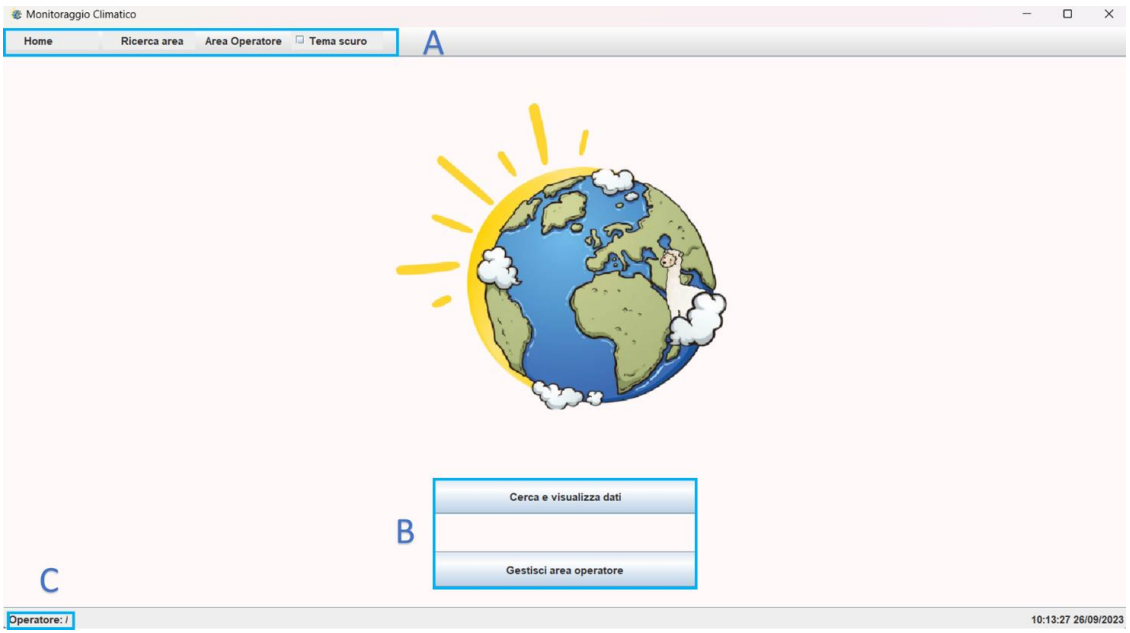
\includegraphics[width=1\textwidth]{../../img/schermata_home.png}
    \caption{Schermata Home}
\end{figure}

\begin{enumerate}
\renewcommand{\labelenumi}{\Alph{enumi}}
    \item \textbf{Barra del menu:} 
    \begin{itemize}
        \item \textbf{Home:} visualizza la schermata principale dell'applicazione senza modificare i dati di accesso dell'operatore corrente.
        \item \textbf{Ricerca area:} permette di accedere alla schermata adibita alla ricerca di un'area specifica.
        \item \textbf{Area Operatore:} permette di accedere alla schermata adibita alla registrazione e accesso per gli operatori.
        \item \textbf{Tema scuro:} permette di attivare o disattivare il tema scuro dell'applicazione.
    \end{itemize} 
    \item \textbf{Pulsanti principali:}
    \begin{itemize}
        \item \textbf{Cerca e visualizza dati:} ha la stessa funzione di \emph{Ricerca area} nella barra del menu.
        \item \textbf{Gestici area operatore:} ha la stessa funzione di \emph{Area Operatore} nella barra del menu.
    \end{itemize}
    \item \textbf{Operaore:} visualizza il nome dell'operatore corrente; se non è stato effettuato l'accesso, verrà visualizzato il carattere /.
\end{enumerate}